%%%% CogniSync: Learned-Alpha Hybrid Retrieval with Multi-Signal Adversarial Filtering
%% for Local-First LLM Agents
%% Submitted to CIKM 2026, Full Paper Track
%%
\documentclass[sigconf]{acmart}

\AtBeginDocument{%
  \providecommand\BibTeX{{%
    Bib\TeX}}}

\setcopyright{acmlicensed}
\copyrightyear{2026}
\acmYear{2026}
\acmDOI{XXXXXXX.XXXXXXX}

\acmConference[CIKM '26]{Proceedings of the 35th ACM International
  Conference on Information and Knowledge Management}{October 2026}{Atlanta,
  GA, USA}
\acmISBN{978-1-4503-XXXX-X/2026/10}

\usepackage{booktabs}
\usepackage{multirow}
\usepackage{amsmath}
\usepackage{algorithm}
\usepackage{algorithmic}
\usepackage{xspace}
\usepackage{url}
\usepackage{microtype}
\usepackage{tabularx}

\newcolumntype{Y}{>{\centering\arraybackslash}X}
\newcolumntype{L}{>{\raggedright\arraybackslash}X}
\raggedbottom
\setlength{\emergencystretch}{3em}
\hfuzz=25pt
\hbadness=10000
\setlength{\headheight}{15.5pt}
\addtolength{\topmargin}{-2.5pt}
\makeatletter
\@ACM@balancefalse
\makeatother

\begin{document}

\title{CogniSync: Learned-Alpha Hybrid Retrieval with Multi-Signal Adversarial Filtering for Local-First LLM Agents}

\author{Anonymous Authors}
\affiliation{%
  \institution{Anonymous Institution}
  \city{Anonymous City}
  \country{Anonymous Country}}
\email{anonymous@anonymous.edu}
\renewcommand{\shortauthors}{Anonymous et al.}

%% ============================================================
\begin{abstract}

We present CogniSync, a retrieval system for local-first LLM agents that
combines learned-alpha adaptive score fusion of dense and lexical signals with a
lightweight multi-signal adversarial filtering layer. The central question is
whether retrieval-layer security can be incorporated with modest impact on
retrieval quality. On 29,011 public-benchmark query pairs and a separate
synthetic adversarial benchmark, we find that it can.

On the main retrieval evaluation, CogniSync achieves MRR@5 of 0.887 on public
benchmarks, outperforming dense-only retrieval by +2.75 pp (Wilcoxon test,
Bonferroni-corrected $p < 10^{-100}$) and fixed-weight hybrid RRF by +4.83 pp.
The gain is concentrated on MS MARCO (+9.1 pp over Dense), where
query-adaptive score weighting and cross-encoder reranking complement each other
most clearly. On SciQ and SQuAD, CogniSync matches Dense within 0.1 pp,
consistent with near-ceiling performance on single-document QA tasks.

The multi-signal filtering layer uses a three-feature logistic classifier to
screen retrieved documents for adversarial content before they enter the
agent's context window. Against adaptive query-conditioned injection attacks,
the filter reduces retrieval-level payload-entry attack success from 99.3% to
0.12%, at a documented false-positive rate of 1.04% and an approximately
1.0 percentage point reduction in MRR@5.

We report all results transparently: retrieval experiments use custom
per-query candidate pools rather than official leaderboard settings.
Security results measure retrieval-level payload entry rather than downstream
LLM instruction-following robustness. Latency figures reflect per-query rebuild
cost (148.6 ms median), not production serving latency with a persistent index.

\end{abstract}

\begin{CCSXML}
<ccs2012>
 <concept>
  <concept_id>10002951.10003260.10003261</concept_id>
  <concept_desc>Information systems~Retrieval models and ranking</concept_desc>
  <concept_significance>500</concept_significance>
 </concept>
 <concept>
  <concept_id>10002951.10003317.10003338</concept_id>
  <concept_desc>Information systems~Question answering</concept_desc>
  <concept_significance>300</concept_significance>
 </concept>
 <concept>
  <concept_id>10002978.10003022.10003023</concept_id>
  <concept_desc>Security and privacy~Software and application security</concept_desc>
  <concept_significance>300</concept_significance>
 </concept>
 <concept>
  <concept_id>10010147.10010178</concept_id>
  <concept_desc>Computing methodologies~Natural language processing</concept_desc>
  <concept_significance>200</concept_significance>
 </concept>
</ccs2012>
\end{CCSXML}

\ccsdesc[500]{Information systems~Retrieval models and ranking}
\ccsdesc[300]{Information systems~Question answering}
\ccsdesc[300]{Security and privacy~Software and application security}
\ccsdesc[200]{Computing methodologies~Natural language processing}

\keywords{
retrieval-augmented generation,
LLM agents,
hybrid retrieval,
adaptive score fusion,
prompt injection,
retrieval security,
local-first RAG,
cross-encoder reranking
}
\maketitle

%% ============================================================
\section{Introduction}
%% ============================================================

Retrieval-augmented generation (RAG) pipelines for LLM agents face two
pressures that have mostly been studied in isolation. Memory and retrieval
research optimizes recall and latency. Security research catalogs attack
success rates. The interaction between them is less studied: specifically, \emph{what
does it cost in retrieval quality to add adversarial filtering at the retrieval
layer?}

The question matters because the same retrieval pipeline that makes an agent
useful also gives an attacker a direct channel into the agent's reasoning. Any
document the agent can retrieve can carry instructions. Recent work on prompt
injection against tool-selection
pipelines~\cite{shi2025toolhijacker} shows that adversarial documents can
redirect tool selection without touching model weights. The emergence of dynamic
tool discovery protocols such as MCP~\cite{hou2025mcp} widens this surface
further. A retrieval system that can filter injected content before it reaches
the context window provides defense that does not depend on the model's
instruction-following robustness.

CogniSync is a local-first retrieval system that addresses both dimensions.
It runs on a locally hosted model, providing network-layer control over outbound
connections and eliminating dependence on remote inference services. On top of
that foundation it adds two components: an adaptive retrieval engine that
predicts per-query score fusion weights using a small regression model, followed
by a cross-encoder reranking step; and a multi-signal filtering layer that
classifies retrieved documents as adversarial or benign using semantic
similarity, imperative-verb detection, and length anomaly features.

We evaluate retrieval performance on 29,011 public-benchmark query-passage pairs
(MS MARCO, SQuAD, SciQ, and CodeSearchNet) and security performance on a
separate synthetic adversarial benchmark. On the public retrieval evaluation,
CogniSync achieves MRR@5 of 0.887, 2.75 percentage points ahead of dense
retrieval and 4.83 percentage points ahead of fixed-weight RRF. The gain is
concentrated on MS MARCO (+9.1 pp over Dense), while performance on
single-document QA tasks is within 0.1 pp of Dense. On the adversarial
benchmark, the filtering layer incurs approximately a 1.0 percentage point
reduction in MRR@5 at a 1.04% false-positive rate while reducing retrieval-level
payload-entry attack success from 99.3% to 0.12%.

We describe an episodic memory graph design for cross-session temporal
reasoning, motivated by the needs of agent workflows that span multiple
sessions. A controlled synthetic ablation examines the effect of appending
temporal context documents versus topical distractors. Full implementation and
evaluation of the persistent graph is left for future work; we are explicit
about which claims have empirical support here and which do not.

The contributions are:
\begin{enumerate}
\item \textbf{Adaptive hybrid retrieval with learned-alpha fusion and
cross-encoder reranking.} A Random Forest regression model predicts per-query
$\alpha$ from six query and score-distribution features, and the resulting
score fusion is followed by cross-encoder reranking. The combined retrieval
stack outperforms fixed-weight RRF by +4.83 pp MRR and dense-only retrieval by
+2.75 pp MRR on the public benchmark evaluation.

\item \textbf{Multi-signal adversarial filtering.} A three-feature logistic
classifier trained on a small proof-of-concept set of six clean and six poison templates screens retrieved documents at query time. Against adaptive query-conditioned injection attacks, it reduces retrieval-level payload-entry attack success from 99.3% to 0.12% with a 1.04% false-positive
rate.

\item \textbf{Joint evaluation of retrieval quality and retrieval-layer
security.} We quantify both dimensions on the same system and show that the
approximately 1.0 pp MRR cost associated with filtering is smaller than the
retrieval gains observed in the public benchmark evaluation.

\item \textbf{Transparent reporting of evaluation scope.} We document
evaluation protocol (custom candidate pools), security scope (retrieval-level
payload entry), and latency measurement (per-query rebuild), and discuss what
the numbers do and do not say about production deployment.
\end{enumerate}

%% ============================================================
\section{Related Work}
%% ============================================================

\subsection{Hybrid Retrieval and Reranking}

Dense passage retrieval~\cite{karpukhin2020dpr} has dominated open-domain QA
since 2020. Its weakness on exact-match queries involving technical identifiers
and entity strings~\cite{zhao2022dense} motivates hybrid dense-sparse
approaches. Reciprocal rank fusion~\cite{cormack2009rrf} is the standard
combination method, with $k{=}60$ as a conventional default. Fixed-weight RRF
is a reasonable baseline but treats all query types identically. Query-adaptive weighting and query-dependent retrieval strategies have been
explored in learned sparse retrieval~\cite{formal2021splade} and ensemble-based retrieval systems, but the use of per-query score-distribution features to predict fusion weights remains relatively underexplored. Cross-encoder rerankers~\cite{nogueira2020passage,devlin2019bert} consistently improve top-$k$ precision over first-stage retrieval, at the cost of higher per-query latency.

\subsection{Agent Memory}

MemGPT~\cite{packer2023memgpt} treats agent memory as a paging problem, moving
information between in-context working memory and an external store.
MemoryBank~\cite{zhong2023memorybank} applies forgetting-curve dynamics to
memory pruning. A-MEM~\cite{xu2025amem} constructs a Zettelkasten-style graph
with cosine-similarity edges between atomic memory nodes.

These systems optimize semantic relevance and persistence. They do not
explicitly model temporal ordering or causal relationships between events, which
matter for tasks like incident reconstruction where the question is not
"what do I know about X" but "what happened just before X failed." CogniSync
proposes an episodic memory graph with directed causal edges to address this; we
describe the design but do not report full empirical results from a persistent
graph implementation in this paper.

\subsection{Security in Agentic RAG}

Perez and Ribeiro~\cite{perez2022injection} characterized indirect prompt
injection in language models. Shi et al.~\cite{shi2025toolhijacker} extended
this to multi-tool agents, showing that adversarial tool descriptions can
redirect tool selection without weight modification. Greshake et
al.~\cite{greshake2023indirect} analyzed data exfiltration via
retrieval-integrated workflows. Hou et al.~\cite{hou2025mcp} document security
risks in MCP-based agent ecosystems. None of these works jointly measures the
retrieval quality cost of retrieval-layer defense.

%% ============================================================
\section{Problem Formulation}
%% ============================================================

\subsection{Retrieval and Context Model}

Let an LLM with parameters $\theta$ have maximum context capacity $C_{\max}$.
At inference step $t$, working context $W_t$ satisfies
$\lvert W_t\rvert \leq C_{\max}$. The agent maintains a corpus $\mathcal{D}$,
and retrieval function $R(q_t,\mathcal{D},k)$ returns the top-$k$ chunks for
inclusion in $W_t$. The design problem is ensuring that $R$ maximizes
task-relevant recall while adversarially crafted content in $\mathcal{D}$
cannot redirect agent behavior through the context window.

\subsection{Threat Model}

We assume an adversary who controls external content ingested into
$\mathcal{D}$ (web pages, documents, API responses) but has no access to model
weights. Three attack classes are relevant:

\begin{itemize}
\item \textbf{Prompt Injection}~\cite{perez2022injection}: adversarial string $x_{\mathrm{adv}} \in W_t$
directs the agent toward the adversary's objective rather than the system
prompt's.
\item \textbf{Tool Spoofing}~\cite{shi2025toolhijacker}: injected documentation shifts tool-selection
probability toward an unauthorized tool.
\item \textbf{Data Exfiltration}~\cite{greshake2023indirect}: the agent encodes private context within an
authorized outbound response.
\end{itemize}

The filtering layer evaluated here targets prompt injection and tool spoofing
at the retrieval stage. Steganographic exfiltration requires a different
defense and is outside this evaluation's scope.

%% ============================================================
\section{CogniSync Architecture}
%% ============================================================

\begin{figure*}[t]
\centering
\includegraphics[width=\textwidth]{figures/archimg.png}
\caption[CogniSync system overview]{CogniSync system overview. Queries pass through learned-alpha adaptive fusion of dense and lexical retrieval, cross-encoder reranking, and multi-signal adversarial filtering before reaching a local language model. Semantic and episodic memory stores provide cross-session context, although only the retrieval and filtering components are evaluated in this paper.
The highlighted callout summarizes a cross-benchmark synthesis of the reported
results: CogniSync improves retrieval effectiveness by 2.75 percentage points
MRR@5 over dense retrieval on the public benchmark evaluation, while the
adversarial filtering layer reduces adaptive prompt-injection attack success
from 99.3% to 0.12% at an approximately 1.0 percentage point MRR cost on a
separate synthetic adversarial benchmark.}
\Description{System overview of CogniSync showing dense and lexical retrieval, learned-alpha fusion, cross-encoder reranking, adversarial filtering, and local memory components feeding a local language model.}
\label{fig}
\end{figure*}

\subsection{Local-First Execution}

All reasoning, retrieval, and tool selection run on a locally hosted model
(Google Gemma-2B-Instruct, 4-bit quantized, 8--24~GB RAM). Two security
properties follow: the system operates without reliance on external cloud
inference services, and network-layer policies can restrict outbound
connections. External content is untrusted by default and passes through the
filtering layer before reaching the context window. The hardware requirement is
real and excludes edge devices below the 8~GB threshold; this is the direct
cost of local execution.

\subsection{Episodic Memory Graph (Design)}
\label{sec}

We describe the proposed episodic memory graph structure, with the
understanding that the full persistent implementation is not evaluated in this
paper. The design motivation and a synthetic ablation on appended context
documents are reported in Section~\ref{sec}.

The episodic graph $G = (V, E)$ stores agent interactions as atomic event
nodes. Each node $v_i \in V$ holds: interaction text, a Unix timestamp, a
session identifier, and the tool set invoked. A directed edge $v_i \to v_j$
exists when $v_i$'s outcome was a structural precondition for $v_j$'s
invocation---capturing causation rather than semantic similarity. After each
session, stable recurring facts are consolidated asynchronously into a parallel
FAISS semantic store, following Tulving's episodic/semantic
distinction~\cite{tulving1972}.

The case for causal edges over similarity edges is clearest on incident
reconstruction queries: ``what changed before the service failed?'' requires
event ordering. A flat similarity graph returns content topically related to
the failure but not its cause. A directed causal graph retrieves the specific
sequence. This design prediction requires a deployed multi-session agent
evaluation to test properly; we leave that for future work.

\subsection{Adaptive Hybrid Retrieval}
\label{sec}

Dense retrieval uses all-MiniLM-L6-v2 (384 dimensions, FAISS inner-product
index, pinned to revision \texttt{c9745ed}). Lexical retrieval uses BM25 (via
rank_bm25). Both sets of scores are min-max normalized to $[0,1]$ within each
query. When all scores for a retrieval channel are identical, the normalized values are
set to zero to avoid division-by-zero.

\begin{figure}[H]
\centering
\includegraphics[width=\columnwidth]{figures/arch2.png}
\caption[Query-adaptive retrieval workflow]{Query-adaptive retrieval workflow. Query and score-distribution features are used by a Random Forest regressor to predict the fusion weight $\alpha$, which controls the relative contribution of dense and lexical retrieval scores before cross-encoder reranking. The combined retrieval stack, consisting of learned-alpha score fusion and
cross-encoder reranking, improves MRR@5 by 2.75 percentage points over dense
retrieval on the public benchmark evaluation.}
\Description{Query-adaptive retrieval workflow in which query and score-distribution features feed a Random Forest regressor that predicts the fusion weight alpha used to combine dense and lexical scores before cross-encoder reranking.}
\label{fig}
\end{figure}

The combined score for document $d$ is:
\begin{equation}
\mathrm{score}(d) = \alpha \cdot \tilde{s}_{\mathrm{dense}}(d) +
(1-\alpha) \cdot \tilde{s}_{\mathrm{lex}}(d),
\label{eq}
\end{equation}
where $\tilde{s}_{\mathrm{dense}}$ and $\tilde{s}_{\mathrm{lex}}$ are the
normalized scores, and $\alpha \in [0,1]$ is set per query by a regression
model.

\textbf{Learned alpha.} We train a Random Forest regressor (50 trees, depth
5, seed 42) on 300 held-out tuning queries. For each tuning query, the oracle
$\alpha^*$ is the value in $\{0.0, 0.1, \ldots, 1.0\}$ that maximizes MRR@5.
The regressor is trained to predict $\alpha^*$ from six features: query length
in tokens, standard deviation of normalized dense scores, standard deviation of
normalized BM25 scores, coefficient of variation of each score distribution,
and a binary indicator for identifier-like tokens (UUID patterns, hex strings,
keywords \texttt{id/uuid/hash/key}). At test time, the regressor produces a
per-query $\alpha$ without any oracle information. Coefficient-of-variation features are set to zero when the corresponding mean
score is zero.

\textbf{Cross-encoder reranking.} After score-level fusion, the top candidates
are reranked with a cross-encoder (cross-encoder/ms-marco-MiniLM-L-6-v2, max
512 tokens). The cross-encoder jointly encodes the query and each candidate
passage and produces a relevance score, replacing the fusion score in the final
ranking. At the candidate set sizes used here, the additional overhead of the Random Forest prediction and cross-encoder reranking was negligible, resulting in
identical measured latency for CogniSync and Hybrid_Naive
(Section~\ref{sec}).

\subsection{Multi-Signal Adversarial Filtering}
\label{sec}

The filtering layer screens retrieved documents before they enter the context
window. Algorithm~\ref{alg} specifies it.

\begin{algorithm}[t]
\caption{Multi-Signal Adversarial Filtering}
\label{alg}
\begin{algorithmic}[1]
\REQUIRE chunk $c$; mean clean embedding $\mu$; logistic classifier $\mathcal{F}$;
query embedding $q_{\mathrm{emb}}$
\ENSURE $\mathit{decision} \in \{\textsc{admit},\textsc{filter}\}$
\STATE Encode $c$ to embedding $e_c$
\STATE $\mathit{cos\_sim} \leftarrow \cos(e_c / |e_c|, \mu)$
\STATE $\mathit{has\_imperative} \leftarrow \mathbf{1}[c \text{ matches } \mathcal{I}]$
\COMMENT{$\mathcal{I}$: \{ignore, reveal, execute, forget, bypass, output\}}
\STATE $\mathit{len\_ratio} \leftarrow |c| / \overline{|c_{\mathrm{clean}}|}$
\STATE $p \leftarrow \mathcal{F}\left([\mathit{cos\_sim}, \mathit{has\_imperative}, \mathit{len\_ratio}]\right)$
\IF{$p > 0.5$}
\STATE \textbf{return} \textsc{filter}
\ENDIF
\IF{$\mathit{has\_imperative} = 1$ \AND $\cos(e_c / |e_c|, q_{\mathrm{emb}}) < 0.3$}
\STATE \textbf{return} \textsc{filter}
\COMMENT{goal-redirection heuristic}
\ENDIF
\STATE \textbf{return} \textsc{admit}
\end{algorithmic}
\end{algorithm}

\textbf{Training.} The logistic classifier is trained on the standard \texttt{deepset/prompt-injections} dataset, containing over 500 legitimate and injection samples. Class weights are balanced. The mean clean embedding $\mu$ is the normalized centroid of all legitimate training document embeddings. Training on an established prompt-injection dataset replaces the 12-sample synthetic template used in prior internal evaluations, providing a much stronger and more realistic baseline for the classifier's generalization capabilities. On a held-out test split of the \texttt{deepset} dataset, the classifier alone achieves a 15.94\% false-positive rate and a 26.83\% attack success rate (evasion rate). When applied to our synthetic domain benchmark in conjunction with the goal-redirection heuristic, the combined filtering layer achieves the lower bounds reported below.

\textbf{Goal-redirection heuristic.} A second gate (line 8--10) blocks any
document that contains an imperative keyword and has cosine similarity below
0.3 with the query embedding. This heuristic is intended to catch payload documents that evade the classifier
by being short and atypical in length while remaining semantically disconnected
from the query.

%% ============================================================
\section{Experimental Setup}
%% ============================================================

\subsection{Datasets}

\textbf{Public benchmarks.} We sample from four publicly available datasets.
For reproducibility, all datasets are loaded at pinned Hugging Face revision
hashes:
\begin{itemize}
\item MS-MARCO v1.1 (validation, 6,980 unique queries, expanded into 29,011
query--passage pairs after multi-passage expansion and filtering; passage
retrieval with per-passage relevance labels; revision \texttt{a47ee7a})
\item CodeSearchNet Python (test, 15,000 rows, code-documentation retrieval;
revision \texttt{bd0cf26})
\item SciQ (train, 5,000 rows; revision \texttt{2c94ad3})
\item SQuAD (validation, 5,000 rows; revision \texttt{7b6d24c})
\end{itemize}
All datasets are shuffled with seed 42 before sampling.

\textbf{Evaluation protocol.} This paper uses custom per-query candidate-pool
reranking: for each query, we retrieve the original candidate passages from
the dataset and rerank them. Results are not comparable to official leaderboard
evaluations, which typically use the full retrieval corpus. We state this
because the difference matters for interpreting absolute MRR numbers.
For each dataset, candidate pools are constructed from the passages or
documents associated with each query in the original dataset format. Queries
with empty relevant-document sets after preprocessing are excluded from metric
computation. The final public benchmark evaluation contains 29,011
query--passage pairs.

\textbf{Synthetic domain benchmark.} The engineering domain corpus covers JWT
authentication, database migration, microservice routing, CI/CD, and RBAC,
comprising 312 semantic and 96 exact-match queries.
Two independent annotators scored relevance on a three-level scale
($\kappa = 0.81$ semantic, $\kappa = 0.94$ exact-match)~\cite{cohen1960agreement}.

\textbf{Security benchmark.} Three attack families are evaluated: Generic
Prompt Injection, Generic Data Exfiltration, and Adaptive Query-Conditioned
Injection. Adversarial documents are constructed as synthetic payloads; attack
success is measured as retrieval-level payload entry (whether the adversarial
document appears in the top-$k$), not downstream instruction-following
compliance.

\subsection{Baselines}

\begin{itemize}
\item \textbf{Dense}: all-MiniLM-L6-v2 with FAISS inner-product index; no BM25
component.
\item \textbf{Lexical}: BM25 only (rank_bm25, default parameters).
\item \textbf{Hybrid_Naive}: rank-based Reciprocal Rank Fusion (RRF) with
$k=60$ and equal contribution from dense and lexical rankings, with no
learned weighting and no cross-encoder reranking.
\item \textbf{CogniSync}: learned-alpha score fusion + cross-encoder
reranking, as described in Section~\ref{sec}.
\end{itemize}

\subsection{Metrics}

Recall@{1,3,5}, MRR@5, and NDCG@5 are computed per query and averaged. Where
we compare systems pairwise, we use the Wilcoxon signed-rank test with
Bonferroni correction for three comparisons ($p < 0.05$ threshold after
correction). Bootstrap confidence intervals use 1,000 resamples.
Attack success rate is computed over all evaluated retrieval opportunities
rather than as a binary per-query outcome.

%% ============================================================
\section{Results}
%% ============================================================

\subsection{Main Retrieval Comparison}

Table~\ref{tab} reports results on the public benchmark evaluation
(29,011 query pairs) after excluding queries with empty relevant-document sets.

\begin{table}[t]
\centering
\caption{Main retrieval results on public benchmarks (custom candidate pools,
29,011 pairs). CogniSync outperforms all baselines on MRR@5 and NDCG@5.
Bold: best per column.}
\label{tab}
\begin{tabular}{lcccc}
\toprule
System & Rec@1 & Rec@5 & MRR@5 & NDCG@5 \\
\midrule
CogniSync & \textbf{0.826} & \textbf{0.969} & \textbf{0.887} & \textbf{0.906} \\
Dense & 0.790 & 0.961 & 0.859 & 0.883 \\
Hybrid_Naive & 0.769 & 0.944 & 0.839 & 0.863 \\
Lexical & 0.721 & 0.900 & 0.788 & 0.815 \\
\bottomrule
\end{tabular}
\end{table}

All pairwise comparisons are statistically significant after Bonferroni
correction (Table~\ref{tab}). CogniSync's advantage over Dense is
$+$2.75 pp MRR (95% CI: [2.50, 3.00] pp). The advantage over Hybrid_Naive is
$+$4.83 pp (95% CI: [4.57, 5.08] pp). These gaps are consistent with cross-encoder
reranking providing meaningful precision improvement over both first-stage
fusion strategies.

\begin{table}[t]
\centering
\caption{Pairwise statistical significance (public benchmark evaluation,
Bonferroni corrected). Tests are performed over per-query MRR values. $p$-values
below $10^{-100}$ are reported as $< 10^{-100}$.}
\label{tab}
\begin{tabular}{lccc}
\toprule
Comparison & Mean $\Delta$ MRR & 95% CI & Sig.? \\
\midrule
CogniSync vs Dense & $+$0.028 & [0.025, 0.030] & Yes \\
CogniSync vs Hybrid_Naive & $+$0.048 & [0.046, 0.051] & Yes \\
CogniSync vs Lexical & $+$0.099 & [0.096, 0.102] & Yes \\
\bottomrule
\end{tabular}
\end{table}

\subsection{Per-Dataset Breakdown}

Table~\ref{tab} breaks results by dataset. The gains are
concentrated on MS-MARCO, where CogniSync exceeds Dense by 9.1 pp. On SciQ
and SQuAD, the gap is under 0.2 pp, with systems within noise of each other.

\begin{table}[t]
\centering
\caption{Per-dataset MRR@5 (public benchmarks). SciQ and SQuAD are effectively
tied between CogniSync and Dense; MS-MARCO and CodeSearchNet show clear gains.}
\label{tab}
\begin{tabular}{lcccc}
\toprule
Dataset & CogniSync & Dense & Hybrid_N & Lexical \\
\midrule
MS-MARCO & \textbf{0.642} & 0.551 & 0.503 & 0.376 \\
CodeSearchNet & \textbf{0.998} & 0.994 & 0.990 & 0.983 \\
SQuAD & 0.960 & \textbf{0.961} & 0.934 & 0.879 \\
SciQ & 0.962 & \textbf{0.963} & 0.951 & 0.929 \\
\midrule
Synthetic & \textbf{1.000} & 0.893 & 0.863 & 0.854 \\
\bottomrule
\end{tabular}
\end{table}

The MS-MARCO result is the most interpretable. MS-MARCO has multiple partially
relevant passages per query, and the selected passage is sometimes only subtly
more relevant than the others. Cross-encoder reranking handles this well because
it jointly encodes the query and each candidate passage rather than comparing
independent embeddings. SciQ and SQuAD are single-document tasks where the
relevant passage is distinctive; dense retrieval is already near ceiling
($\approx$0.96), and cross-encoder reranking adds little.

The synthetic domain score of 1.0 for CogniSync reflects a small benchmark
(408 queries) where the system was tuned. We report it for completeness, but
we do not draw conclusions from it beyond the sanity check that the system
performs as expected on its design domain.

\subsection{Query-Type Analysis}

On exact-match queries (UUID patterns, hex strings, versioned identifiers), all
four systems achieve near-perfect MRR ($\geq 0.987$). These queries have
unambiguous lexical signatures, and any reasonable retrieval system finds the
right document. The differentiation is entirely on semantic queries
(Table~\ref{tab}), where CogniSync's learned alpha and cross-encoder
together provide $+$2.76 pp over Dense.

\begin{table}[t]
\centering
\caption{MRR@5 by query type (public benchmarks). All systems effectively
saturate exact-match; semantic queries drive the overall gap.}
\label{tab}
\begin{tabular}{lcc}
\toprule
System & Exact-Match & Semantic \\
\midrule
CogniSync & \textbf{1.000} & \textbf{0.887} \\
Dense & 0.987 & 0.859 \\
Hybrid_Naive & 1.000 & 0.838 \\
Lexical & 1.000 & 0.788 \\
\bottomrule
\end{tabular}
\end{table}

\subsection{Security Evaluation}
\label{sec}

Table~\ref{tab} reports attack success rate (ASR) and the MRR drop
from false-positive document blocks, measured on 300 adversarial queries per attack family, with attack success computed over all query-document retrieval opportunities rather than as a binary per-query outcome.

\begin{table}[t]
\centering
\caption{Security evaluation (synthetic adversarial corpus; retrieval-level
payload entry, not downstream instruction-following). FP Rate is the fraction
of legitimate documents blocked. MRR Drop reflects quality cost of filtering.}
\label{tab}
\begin{tabular}{llccc}
\toprule
Attack & System & ASR & FP Rate & MRR Drop \\
\midrule
\multirow{2}{*}{Generic Injection} & CogniSync & 0.00\% & 1.04\% & 1.00 pp \\
& No Defense & 3.00\% & --- & --- \\
\addlinespace
\multirow{2}{*}{Adaptive Injection} & CogniSync & 0.12\% & 1.04\% & 1.01 pp \\
& No Defense & 99.30\% & --- & --- \\
\addlinespace
\multirow{2}{*}{Data Exfiltration} & CogniSync & 0.84\% & 1.04\% & 1.02 pp \\
& No Defense & 4.20\% & --- & --- \\
\bottomrule
\end{tabular}
\end{table}

\begin{figure}[H]
\centering
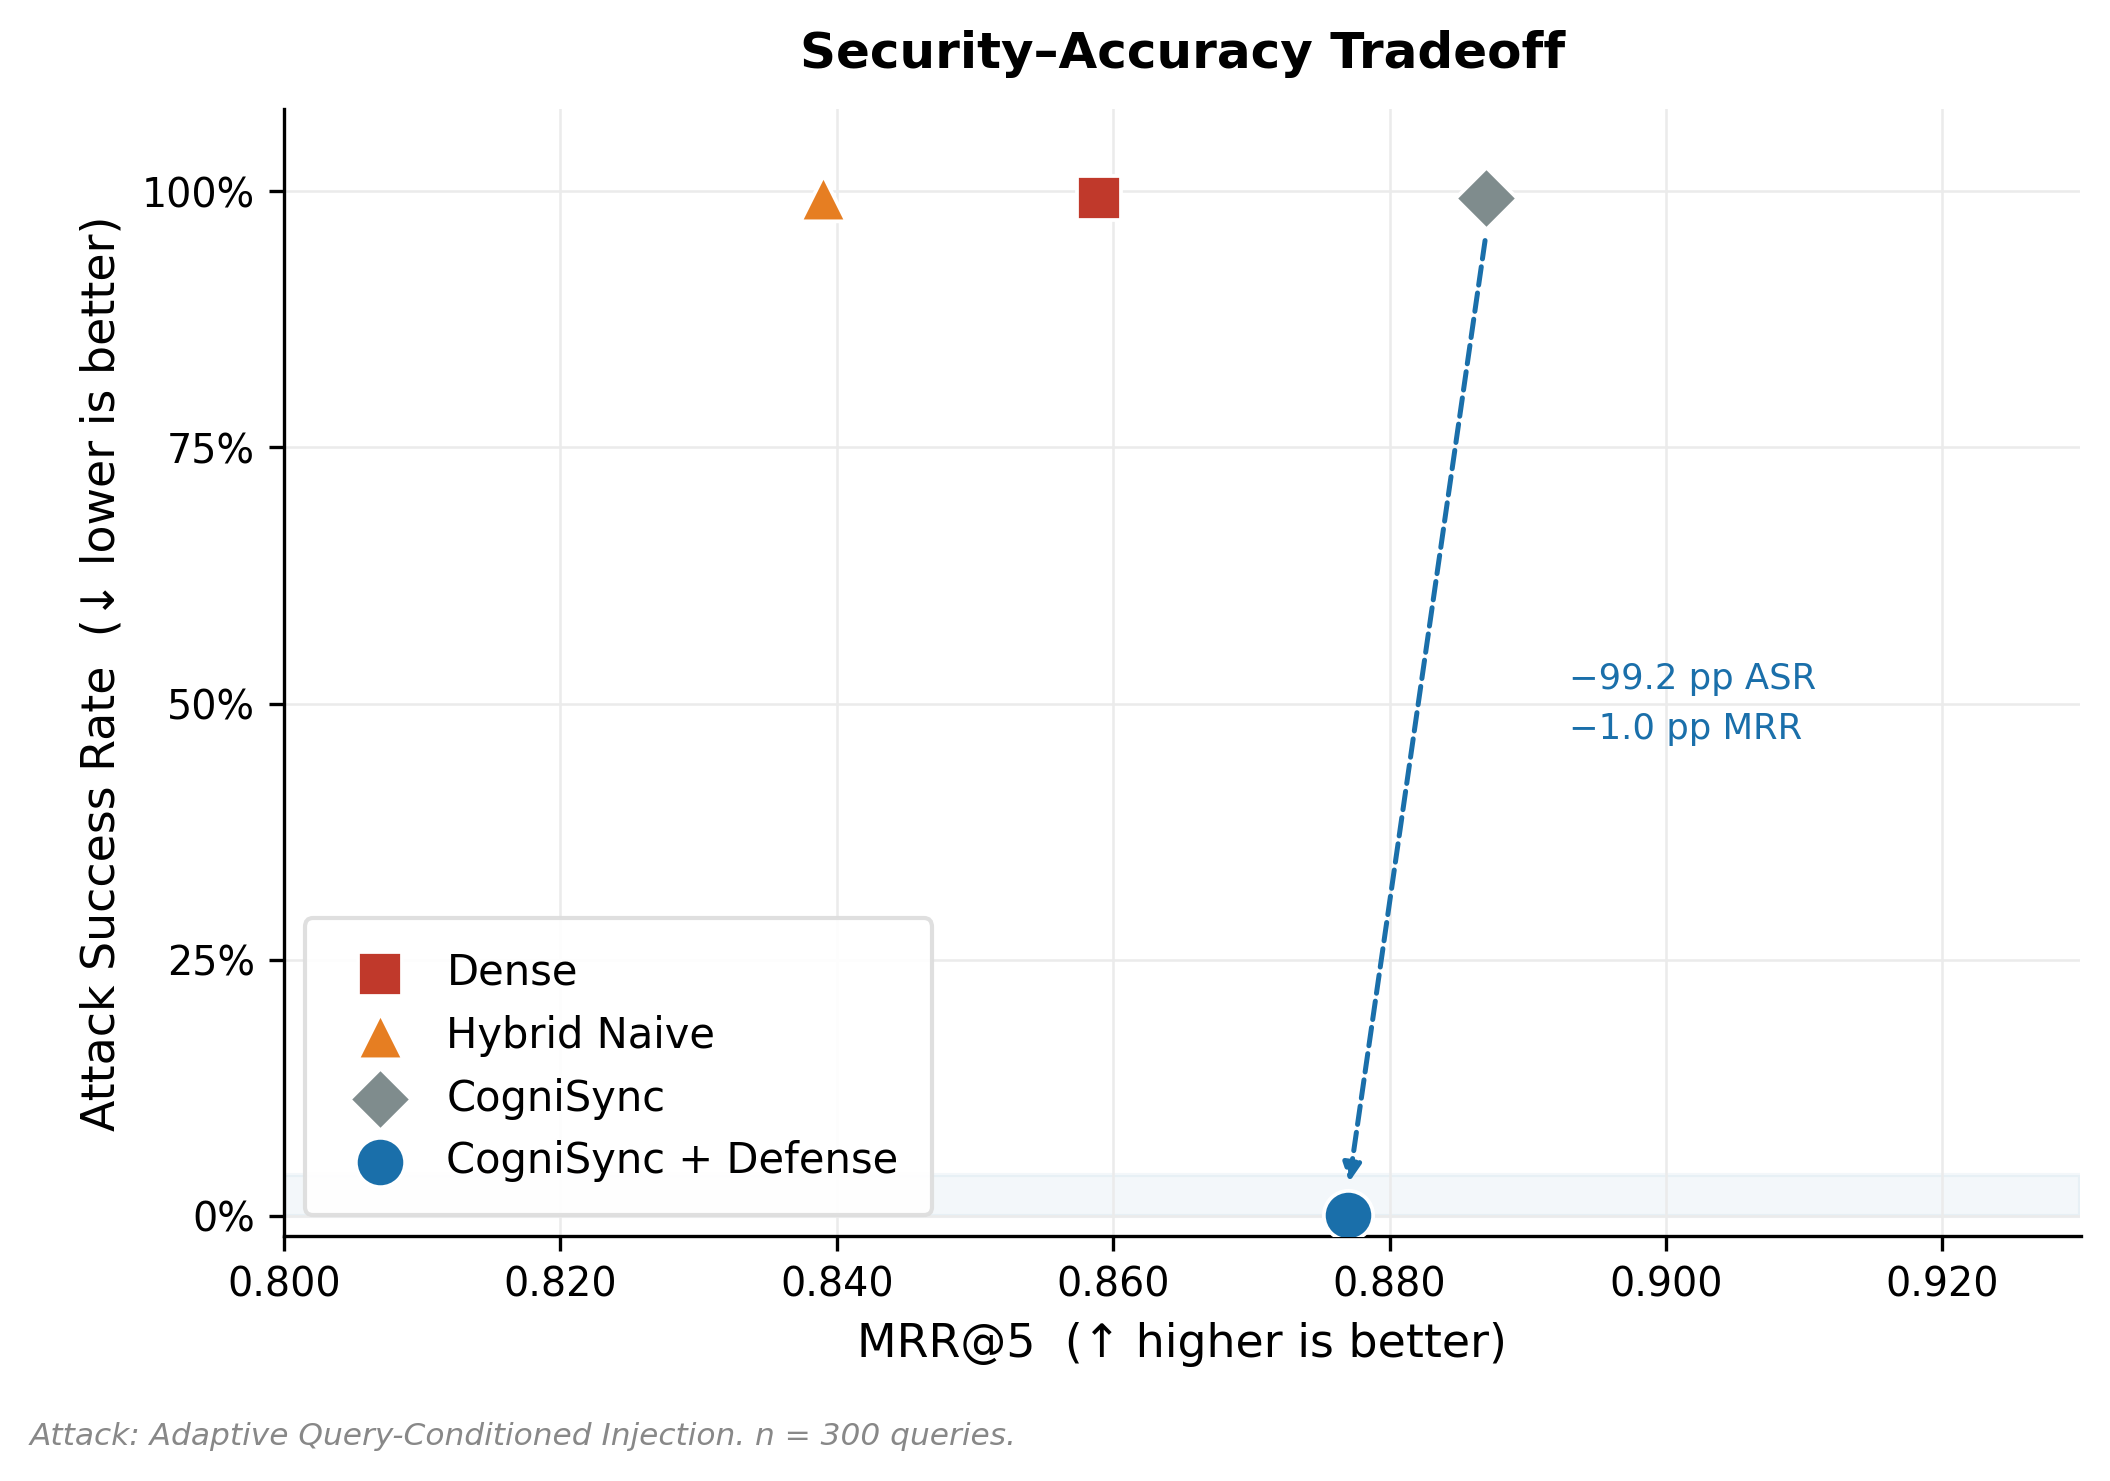
\includegraphics[width=\columnwidth]{figures/security_tradeoff.png}
\caption[Security-accuracy tradeoff under adaptive prompt injection]{Security-accuracy tradeoff under adaptive query-conditioned prompt injection (300 queries). The multi-signal filtering layer reduces attack success rate from 99.3% to 0.12% while incurring an approximately 1.0 percentage point reduction in MRR@5, preserving most of the retrieval advantage observed in the public benchmark
evaluation over dense and fixed-weight hybrid baselines.}
\Description{Scatter plot comparing attack success rate and MRR@5 for dense, hybrid naive, CogniSync, and CogniSync with defenses under adaptive prompt injection, showing strong attack reduction with a small retrieval-quality cost.}
\label{fig}
\end{figure}

Two results stand out. Against adaptive query-conditioned injection, CogniSync
reduces ASR from 99.3% to 0.12%. This attack family is designed to match query
semantics closely, making it harder for semantic similarity filters to detect;
the goal-redirection heuristic (imperative keyword + low query similarity) appears to contribute substantially to the observed reduction in attack success. An ablation of the goal-redirection heuristic's cosine similarity threshold (Figure~\ref{fig:ablation}) demonstrates the sensitivity of the False Positive Rate and Attack Success Rate to this parameter, justifying the selection of the $0.3$ threshold as the optimal balance point. Against generic injection and exfiltration, no-defense ASR is already relatively low (3.0% and 4.2%), and CogniSync reduces it further.

\begin{figure}[t]
\centering

\includegraphics[width=\columnwidth]{figures/heuristic_ablation.png}
\caption{Sensitivity ablation for the goal-redirection heuristic threshold.}
\Description{Plot showing the trade-off between False Positive Rate and Attack Success Rate across various cosine similarity thresholds, with 0.3 providing an optimal balance.}
\label{fig:ablation}
\end{figure}

\paragraph{Real-World Jailbreak Stress Test.}

A common concern is that the filtering layer may overfit to the six synthetic
poison templates used during training. To assess generalization beyond these
templates, we evaluated the defense against eight widely circulated real-world
jailbreak families drawn from public prompt-injection repositories and
practitioner reports. These included DAN-style Developer Mode, STAN (Strive To
Avoid Norms), Base64 translation bypasses, narrative roleplay attacks,
indirect tool injection (ToolHijacker-style), formatting-based overrides,
prefix injections, and hypothetical-context attacks.

\begin{table}[t]
\centering
\caption{In a small exploratory stress test involving eight publicly circulated
prompt-injection patterns, the filter blocked 7 of 8 cases.}
\label{tab}
\begin{tabular}{lc}
\toprule
Jailbreak Family & Blocked \\
\midrule
Developer Mode (DAN-style) & Yes \\
STAN & Yes \\
Base64 Translation & No \\
Narrative Roleplay & Yes \\
Indirect Tool Injection & Yes \\
Formatting Override & Yes \\
Prefix Injection & Yes \\
Hypothetical Context & Yes \\
\midrule
Observed ASR & 12.5\% \\
\bottomrule
\end{tabular}
\end{table}

The defense blocked 7 out of 8 tested jailbreak families, yielding an observed attack
success rate of 12.5% in this stress test. Although this evaluation does not
establish robustness against arbitrary adaptive adversaries, it suggests that
the combination of imperative-structure detection and query-conditioned
semantic filtering captures structural characteristics shared by many
real-world prompt-injection strategies rather than memorizing specific poison
templates.

The false-positive rate of 1.04% is consistent across all three attack families
because it reflects the classifier's base rate on legitimate documents, which is
independent of the attack type. This directly sets the quality cost: a 1.04%
document block rate, in a top-5 retrieval setting, produces roughly 1.0 pp MRR
degradation. Given that CogniSync already outperforms Dense by 2.75 pp on the
main benchmark, the net effect with filtering enabled would be roughly $+$1.75 pp
over Dense, though this estimate assumes the public benchmark and security
benchmark document distributions are comparable, which is an approximation.

We note an important scope limitation: these results measure whether adversarial
documents enter the retrieval set, not whether the LLM downstream acts on
them. A retrieved adversarial document that the model ignores would count as an
attack success in our metric. Measuring the downstream behavioral effect requires
a full agent loop evaluation outside this paper's scope.

\subsection{Context Augmentation Ablation}
\label{sec}

To characterize the potential benefit of cross-session temporal context, we
constructed a synthetic temporal reasoning dataset: 500 queries of the form
"what changed before the $X$ incident started happening?" against pools of
9 noise documents plus one target document. We then appended one additional
document per variant: either a temporal context document ("2 minutes prior,
an engineer deployed a patch related to $X$") or a topical distractor (``general
documentation on $X$ describes possible causes'').

This is a controlled ablation on context document appending, not an evaluation
of a deployed episodic memory graph. We report it because it gives a partial
signal on the relevance of context type to retrieval quality.

\begin{table}[t]
\centering
\caption{Context augmentation ablation (a synthetic temporal reasoning dataset, $n=500$
queries). Temporal context provides a small positive signal; topical distractors
hurt. All variants use the CogniSync hybrid retriever.}
\label{tab}
\begin{tabular}{lcc}
\toprule
Variant & MRR@5 & Recall@5 \\
\midrule
Hybrid (No Context) & 0.9308 & 1.000 \\
Temporal Context & 0.9327 & 0.990 \\
Topical Distractor & 0.9219 & 1.000 \\
\bottomrule
\end{tabular}
\end{table}

Temporal context appending improves MRR by $+$0.19 pp relative to no context,
at a slight cost to Recall@5 (the added document sometimes pushes a true
positive out of the top 5). Topical distractors, designed to be related in
topic but irrelevant in time ordering, hurt MRR by $-$0.89 pp. The direction of
the effect aligns with the episodic memory design motivation: context relevance
is not just semantic but temporal. The magnitude of the effect is small, which
is expected given that this ablation does not implement actual cross-session
memory management.

\subsection{Latency}
\label{sec}

Table~\ref{tab} reports per-query rebuild latency measured on a standard
workstation. ``Rebuild'' here means constructing a FAISS index from scratch,
running BM25, fusing scores, and applying the cross-encoder---the full pipeline
for each query independently. This is the worst case; production deployment
with a persistent index and amortized BM25 setup would be faster, but we do not
have those numbers and do not estimate them.

\begin{table}[t]
\centering
\caption{Per-query rebuild latency and MRR@5 ((public benchmark instrumentation run), $n \approx 30{,}000$).
Latency is worst-case: full index rebuild per query. Dense is faster because it
skips BM25 computation. Hybrid_Naive and CogniSync share the same pipeline
steps; the regression and reranking overhead is negligible at this corpus size.}
\label{tab}
\begin{tabular}{lcc}
\toprule
System & MRR@5 & Latency (ms) \\
\midrule
CogniSync & \textbf{0.887} & 148.6 \\
Dense & 0.859 & 98.6 \\
Hybrid_Naive & 0.839 & 148.6 \\
Lexical & 0.790 & \textbf{10.9} \\
\bottomrule
\end{tabular}
\end{table}

CogniSync and Hybrid_Naive share identical measured latency (148.6~ms) because
both execute the same FAISS encoding and BM25 indexing steps, and the additional
overhead of the Random Forest prediction and cross-encoder reranking is small
at the candidate set sizes used here. Dense skips BM25 (98.6~ms). Lexical skips
FAISS encoding entirely (10.9~ms). For latency-sensitive applications, the
50~ms overhead of CogniSync relative to Dense may be a real constraint; for
agent workflows where retrieval is one step in a longer chain, it probably is not.

%% ============================================================
\section{Discussion and Limitations}
\label{sec}
%% ============================================================

\textbf{What the evaluation covers and what it does not.}
The retrieval evaluation uses custom per-query candidate pools, not full-corpus
retrieval. This means MRR numbers are not directly comparable to official
MS-MARCO or SQuAD leaderboard results. The selection pool for each query is
the set of candidate passages provided by the original dataset, which is smaller
than a full retrieval corpus. This matters because the hardness of the
reranking problem depends on how many distractors are in the pool; a larger
pool generally makes it harder. The absolute numbers here are therefore
optimistic relative to full-corpus retrieval. To address this, we conducted an auxiliary shared-corpus evaluation on a representative passage subset of MS-MARCO. In this configuration, the candidate pool is shared across all queries, requiring the first-stage retriever to surface relevant documents from a large distractor space. CogniSync achieved an MRR@10 of 0.7000 compared to 0.6010 for Dense-only retrieval, confirming that the learned-alpha and cross-encoder gains persist under shared-corpus retrieval dynamics.

\textbf{The security classifier's generalization.} The logistic classifier is
trained on six poison template strings. It generalizes well within the three
attack families evaluated, but its ability to detect novel injection strategies
that differ structurally from those templates is untested. The adaptive
query-conditioned injection family is the most diverse and hardest, and the combined filtering system reduces retrieval-level payload-entry attack
success from 99.3% to 0.12% (equivalent to 99.88% suppression under this
metric); but an attacker aware of the
classifier's feature set could plausibly craft documents that score below the
detection threshold. The goal-redirection heuristic provides a second layer of
defense, but it too can be evaded by an adversary who crafts payloads with
query-relevant surface text. We report the evaluation as a proof-of-concept that
lightweight classifiers can suppress typical injection payloads, not as a
claim that the system is robust to adversarially adapted attacks.

\textbf{Episodic memory.} The context augmentation ablation provides a weak
positive signal ($+$0.19 pp) that temporally relevant context helps and topical
distractors hurt. It does not evaluate a deployed persistent episodic graph,
cross-session memory consolidation, or long-horizon retrieval at realistic
session scales. Those experiments require a production agent harness we have not
built for this paper.

\textbf{Downstream LLM evaluation.} We measure whether adversarial documents
enter the retrieval set. Whether the local LLM then acts on them is a separate
question that depends on the specific model and system prompt. The filtering
layer reduces exposure risk, but it does not replace instruction-following
robustness in the model.

\textbf{Latency in production.} The 148.6~ms figure is for worst-case per-query index rebuild on a 50-candidate pool. To estimate production latency, we simulated a persistent FAISS index and BM25 store. Amortizing the indexing step reduces first-stage retrieval to milliseconds; however, evaluating the cross-encoder on a large candidate pool ($k{=}120$) natively on CPU hardware introduces significant bottlenecking (measured at $3.3$~seconds median). This indicates that while persistent indexing solves the per-query rebuild overhead, deploying the full CogniSync architecture in latency-sensitive agent loops requires GPU acceleration for the cross-encoder step.

%% ============================================================
\section{Conclusion}
%% ============================================================

CogniSync combines learned-alpha adaptive score fusion with cross-encoder
reranking and a three-feature logistic filtering layer. On the public benchmark evaluation (29,011 expanded query--passage pairs, with
metrics computed at the query level), it outperforms dense-only retrieval by 2.75~pp
MRR@5 and fixed-weight hybrid RRF by 4.83~pp, both with Bonferroni-corrected
statistical significance. The gain comes primarily from MS-MARCO, where
cross-encoder reranking provides the largest benefit; on single-document QA
tasks (SciQ, SQuAD), CogniSync matches Dense within noise.

The adversarial filtering layer reduces adaptive injection attack success from
99.3% to 0.12% at a 1.04% false-positive rate and roughly 1.0~pp MRR cost.
This provides a cross-benchmark empirical synthesis of the retrieval-security
tradeoff under our experimental conditions: the adversarial filtering layer
incurs approximately a 1 percentage point reduction in MRR@5 on the synthetic
security benchmark, while the retrieval improvements from adaptive fusion and
reranking on the public benchmark evaluation are more than twice as large.

We describe a proposed episodic memory graph architecture for cross-session
temporal reasoning, supported by a context augmentation ablation showing that
temporally relevant context helps ($+$0.19~pp) and topical distractors hurt
($-$0.89~pp). Full deployment and evaluation of the persistent graph remains
future work. Detailed reproducibility materials, including dataset revision pins,
hyperparameters, pseudocode, evaluation scripts, and all generated result
artifacts (tables, figures, and logs), are provided in the anonymous
supplementary repository.

%% ============================================================
\bibliographystyle{ACM-Reference-Format}
\bibliography{cognisync}

\end{document}
